

%%% This LaTeX source document can be used as the basis for your technical
%%% report. Intentionally stripped and simplified
%%% and commands should be adjusted for your particular paper - title, 
%%% author, citations, equations, etc.
% % Citations/references are in report.bib 

\documentclass[conference,backref=page]{acmsiggraph}
\usepackage{listings}
\TOGonlineid{45678}
\TOGvolume{0}
\TOGnumber{0}
\TOGarticleDOI{1111111.2222222}
\TOGprojectURL{}
\TOGvideoURL{}
\TOGdataURL{}
\TOGcodeURL{}

% Include this so that citations show up in blue and the page information is included in the reference section
\hypersetup{
    colorlinks = true, 
    linkcolor = blue,
    anchorcolor = red,
    citecolor = blue, 
    filecolor = red, 
}


\title{Mesh Destruction\\
	   Final Report}

\author{Students Name \thanks{e-mail:40167111@live.napier.ac.uk} \\
Edinburgh Napier University\\
Physics-Based Animation (SET09119)}
\pdfauthor{Conner Weatherston}

\keywords{Rigid body, collision detection, bounding volumes, mesh destruction, OpenGL, real-time, physics, computer graphics}

\begin{document}

\teaser{
   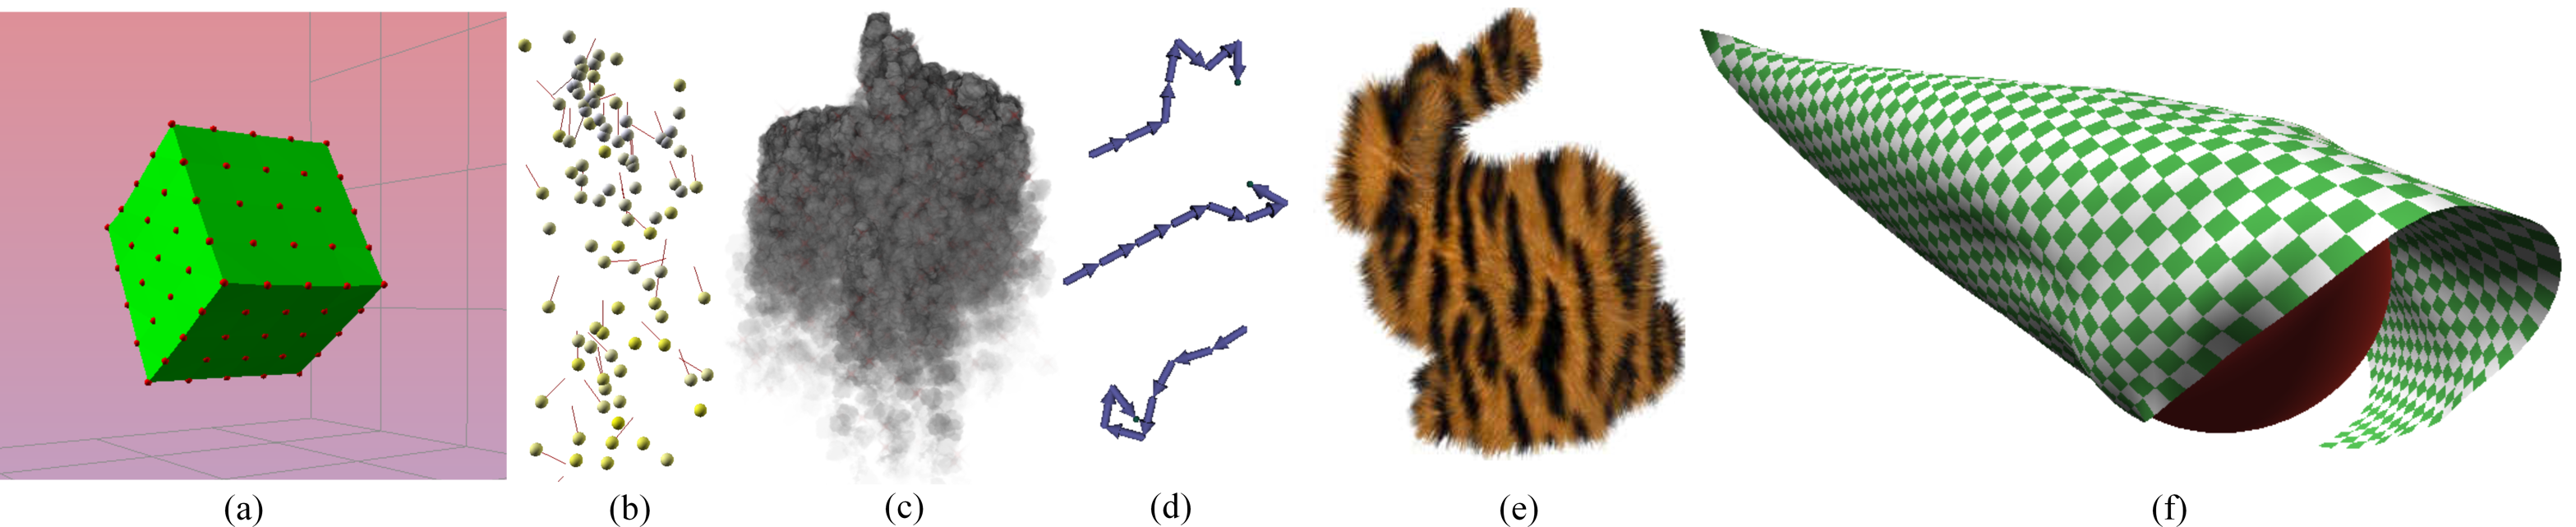
\includegraphics[height=1.5in]{images/sampleteaser}
   \caption{Place a teaser image at the top of your report to show key examples of your work (e.g., multiple screenshots of the different test situations) - Every figure should have a caption and a description.  For example, each figure is labelled and explained: (a) soft bodies, (b) particles, (c) inverse kinematics, (e) fur shells, and (f) position-based dynamics for cloth effects.}
   \label{fig:teaser}
 }

\maketitle

\raggedbottom

\begin{abstract}
In most physics based games, any destructible objects are normally loaded in with their fractured components on runtime. What this
physics simulation is hoping to look at is ways to slice meshes in real time to generate new fragments.

The approach looked at the in the design report suggested a technique called voronoi shattering in order to break the objects up into random fragments. However this was not implemented in the final simulation due to difficulty and time constraints. Therefore a simpler approach was used where the object is split is recursively using a series of random planes which intersect through the model mesh.

\end{abstract}



\keywordlist


\section{Introduction}

In most video games, destructible objects are pre-computed models which are the equivalent of the model fragments. The purpose of this simulation is to create proper mesh fragments in real-time just using the original meshes information. A key part of this simulation is optimisation as creating new objects is an expensive process.  

\section{Related Work}

Currently there are several plugins that use either the same idea or
has a similar solution. However these are mostly implemented into
modelling software where optimisation is not an issue as it is not
required in a real-time environment. The most similar idea is the
plugin by [Esteve 2011]. The tutorial provided gave a insight on how to split the meshes by using planes.

\section{Simulation}

\paragraph{Overview}


\paragraph{Detailed description}

\paragraph{Implementation}

The implementation of this project can be broken into three major segments. These are: rigid bodies, collision detection and meshes. 

\paragraph {Collision detection} \hfill

There are three types of colliders that are used in this simulation. These are the plane collider, the sphere collider and the orientated bounding box.


\subparagraph{Collider} \hfill

This is the basic collider, which every other collider will inherit from. As it is the most general form it only contains a position.

\begin{lstlisting}
Class Collider
{
	Vect3 position;
	
	// This is used to update the position of the colliders.
	void Update(); 
}
\end{lstlisting}

\subparagraph{Plane collider} \hfill

The plane collider is used to simulate the floor. However as the floor is not meant to have true rigid body properties. i.e it should not 'fall' as it will never move, therefore there is a plane collider and a graphic drawn for it rather than it being a true 'Model' object in the scene.

\begin{lstlisting}
Class PlaneCollider : public Collider
{
	Vec3 normal;
}
\end{lstlisting}

\subparagraph{Sphere collider}  \hfill 

This is a simple sphere which encompasses the entire model object. It only requires a position in the world, which is updated whenever the rigid body is updated, and a radius. The radius is calculated by finding the distance from the centre of the model to its furthest point. 

\begin{lstlisting}
Class SphereCollider : public Collider
{
	float radius;
}
\end{lstlisting}

\subparagraph{Orientated bounding box}\hfill 

This is similar to an axis aligned box however it can handle rotations. Detecting collisions for an OBB however is more cost as there are more potential ways two OBB can collide. Therefore, in order to minimise calculations, the OBB checks only occur if both object pass the sphere collider check. 

\begin{lstlisting}
Class BoundingBox : public Collider
{
	float topX,topY,topZ;
	float botX,botY,botZ;
}
\end{lstlisting}
With the 6 points provided the corners of the box can be easily computed.


\subparagraph{Intersections}


\paragraph{Rigid bodies} \hfill

In order to have a simulation which simulates proper physics, rigid bodies need to be attached to the objects. An rigid body consists of the following: position, previous position, mass, inverse mass, orientation, forces being applied to the object. 


\paragraph{Meshes}

\paragraph{Update} \hfill

To create an realistic simulation a concept of a 'physics tick' is required. This is in place in order to decouple the physics from the frame-rate. Thus the physics will run the same if the frame rate is at 10 FPS or 60 FPS.  

There are three parts to the physics update. There are summerised below:

\subparagraph{Colliding object}
The first stage is detecting if any objects are currently colliding with each other.
If there is a collision between two objects then a struct called 'CollisionInfo' is created which contains the following data:

\begin{itemize}
\item{Pointer to object A.}
\item{Pointer to object B.}
\item{Depth of overlap in objects.}
\item{Direction to be pushed towards.}
\item{Position of collision.}
\end{itemize}

This struct is then pushed back onto a vector; which contains all the collisions that have happened between the models in this current update.
\subparagraph{Resolve collisions}\hfill

For each of the collisions that have occurred a resolve stage needs to occur. This calculates what should happen to each object in terms of direction it is now going; the velocity of the objects and if the proper conditions have been met, one of the objects shatter.
\subparagraph{Integrate rigid bodies}\hfill

After collisions have been sorted, each model need to update there current position, previous position, orientation.

% EVALUATION
\section{Testing and evaluation}


\section{Conclusion and Future work}
To conclude, I am done.
% \section*{Acknowledgements}


\bibliographystyle{acmsiggraph}
\bibliography{report}

\end{document}

